% =========================================================================
% Suggested update of ch4_IPCresults_orig.tex (same structure).
% Data and figures: Combined-IPC-TEFC-for-Load-Reduction-of-Wind-Turbines,
%   Main/plotFunktionen/plotIPC_RateLimitComparison.m (dataSet "fadeIn"),
%   which writes Main/plotFunktionen/figIPCThesis/fig00a_Timeseries1/2/3,
%   fig02_PSDroot_breaky_ratecomp (.eps/.png) and tab_stddev_unified_IPC.tex.
%   Copy these figures to figures/figIPCThesis/ in the thesis repository.
% IPC gains: fmincon results of the re-optimization with the IPC/TEF
%   fade-in (Results_IPC_PI_RateLimitOpt/FadeIn/best.mat).
% Wind: TurbKlasseA/18mps.bts of the AALC optimization (training) dataset,
%   660 s, evaluated from 66 s.
% =========================================================================
\subsection{Results} \label{subsection: IPCResults}
The IPC gains are tuned separately for each pitch rate limit with a single wind field, which is taken from the optimization dataset that is also used for training the combined IPC-TEFC controller in Section~\ref{sec:CombinedIPC-TrailingEdgeFlapControl}: the turbulent wind field with a mean wind speed of 18\,m/s and turbulence class~A (16\%). The simulations run for 660\,s. The IPC is faded in between 20\,s and 30\,s, and all criteria are evaluated from 66\,s onward, so that the start-up of the simulation does not influence the results. The proportional and integral gains are optimized with the sequential quadratic programming algorithm of MATLAB's \textit{fmincon.m}, minimizing the cost function in Equation~\eqref{eq:costFunIPC} subject to the constraint that the tower base DEL must not exceed that of the baseline controller. The resulting gains are $K_P = 0.2533$, $K_I = 0.1033$ for 4\textdegree/s, $K_P = 1.2219$, $K_I = 0.3702$ for 8\textdegree/s, and $K_P = 1.2227$, $K_I = 0.3653$ for 13\textdegree/s. The gains for 8\textdegree/s and 13\textdegree/s are nearly identical, since the controller optimized for 8\textdegree/s already reaches the rate limit only rarely, as discussed below.

Figure~\ref{fig:timeseriesIPC} visualizes the results of the baseline CPC and two IPC controllers, with parameters optimized for the 4\textdegree/s and 13\textdegree/s pitch rate limits. In all test cases, the turbine is excited with the same wind signal, i.e., the wind field used for the controller tuning. The first subplot shows the wind speed signal. The subsequent plots display pitch angles, pitch rates, rotor speed, tower fore-aft acceleration, generator power, and blade root out-of-plane moments. The generator torque is not shown, as it is constant at its rated value in this Region~III test case for all controllers.
\begin{figure} [H]
    \subfloat[Pitch rate limit 4\textdegree/s]{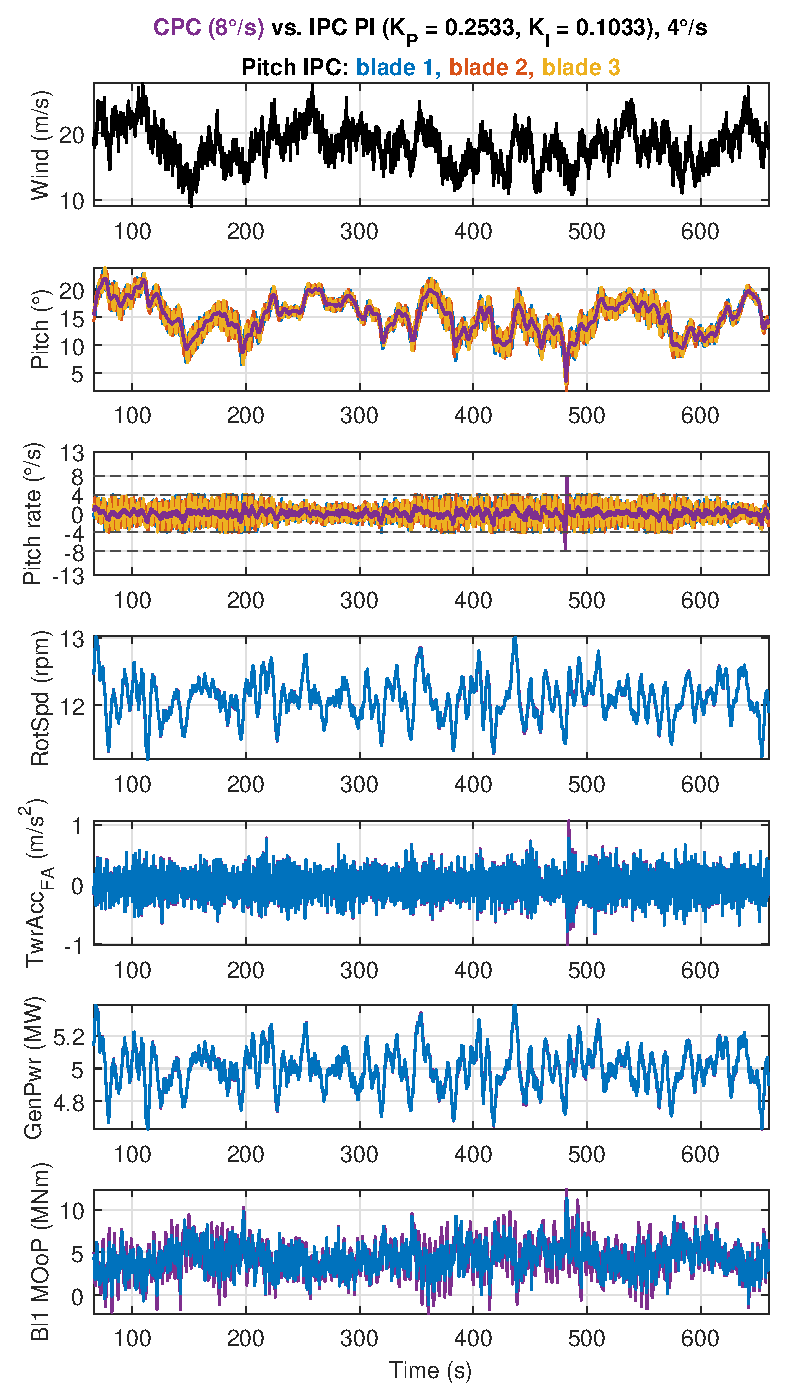
\includegraphics[width=0.49\textwidth]{figures/figIPCThesis/fig00a_Timeseries1.eps}}\hfill
    \subfloat[Pitch rate limit 13\textdegree/s]{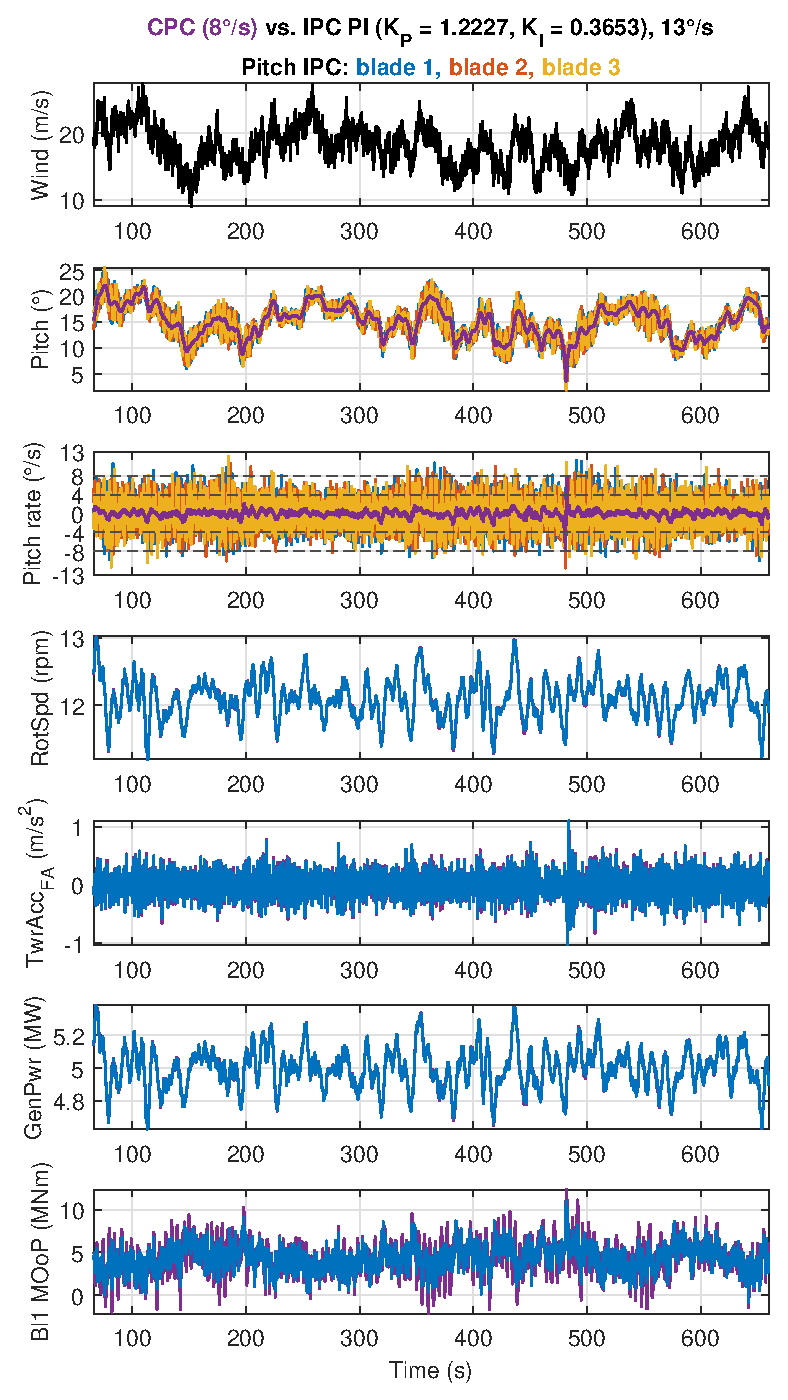
\includegraphics[width=0.49\textwidth]{figures/figIPCThesis/fig00a_Timeseries3.eps}}\hfill
    \caption[Controller comparison: Baseline and IPC PI with different pitch rate limits.]{Controller comparison: Baseline CPC (purple) and IPC PI (blue, red and yellow lines pitch signals of blades 1 to 3, blue all other signals) with different pitch rate limits for turbulent wind (18\,m/s mean, IEC turbulence class A (16\%), wind field of the optimization dataset). Rate limits: Low (4\textdegree/s) and high (13\textdegree/s) for IPC, standard  (8\textdegree/s) for baseline PI. Dashed lines in the pitch rate plots: $\pm 4$\textdegree/s and $\pm 8$\textdegree/s. Displayed signals: wind speed, pitch, pitch rate, states, power, and out-of-plane blade root moments.}
    \label{fig:timeseriesIPC}
\end{figure}

Rotor speed and generator power remain nearly unchanged between the two IPC configurations and the baseline PI CPC. This is expected, as the power control logic, which sets the generator torque and collective pitch demand, is identical across all controllers. Differences in tower fore-aft motion are also nearly imperceptible in this time series. The most notable differences appear in the pitch signals, which oscillate at the 1P frequency in both IPC cases, and in the resulting blade root out-of-plane moments. At the lower pitch rate limit of 4\textdegree/s, shown in the left column, the pitch rates of the IPC frequently reach the limit, i.e., during 2.2\% of the time, which limits the amplitude of the 1P pitch oscillations and thus also the effect of the IPC on the blade root out-of-plane moments. In contrast, the right column, corresponding to the very high pitch rate limit of 13\textdegree/s, shows larger pitch rates that exceed 8\textdegree/s only in short episodes, while the limit of 13\textdegree/s itself is never reached. Here the individual pitch actuators significantly reduce the variance of the out-of-plane moments, thereby improving load reduction on the blades.
As expected, increasing the allowable pitch rate enhances the effectiveness of the IPC controller in alleviating structural loads. Above 8\textdegree/s, however, a further increase of the rate limit brings hardly any additional benefit for this test case.

Figure~\ref{fig:PSDIPC} shows the Power Spectral Density (PSD) of the blade root out-of-plane moment to visualize and explain the gradual improvement with increasing pitch rate for all three test cases. The black line represents the baseline CPC. The blue line, representing IPC with a 4\textdegree/s rate limit, reduces the 1P peak by 91\%, while the red line, representing IPC with an 8\textdegree/s rate limit, further lowers it, achieving a 96\% reduction. At the 2P frequency, the blue line shows only a small decrease of 11\% compared to the baseline, while the red line lowers the 2P peak by 44\%. As expected, the 8\textdegree/s rate limit offers better load reduction across both 1P and 2P frequencies. The controller tuned with the rate limit set to 13\textdegree/s, depicted as a yellow line, lies almost on top of the red line, with 1P and 2P peak reductions of 96\% and 45\%, respectively.
\begin{figure}[h]
    \begin{center}
        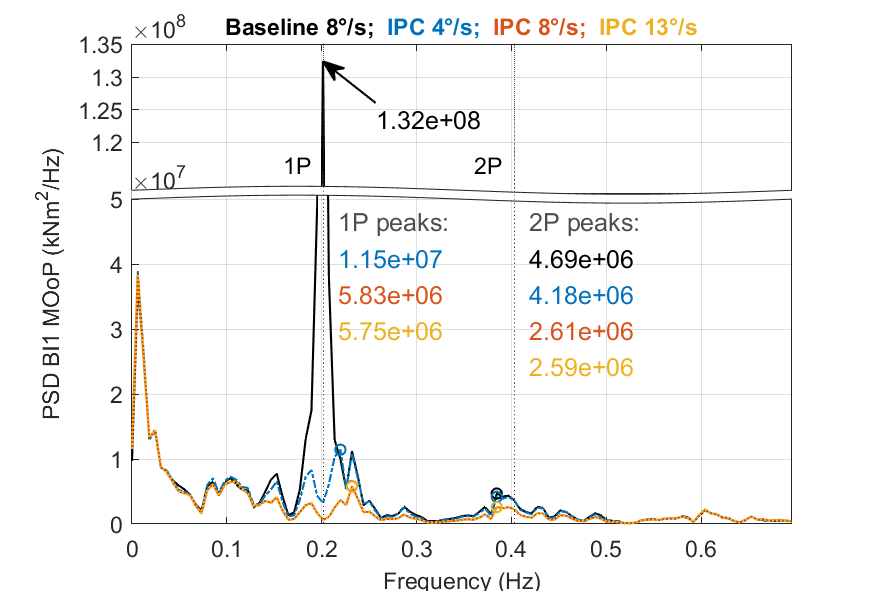
\includegraphics[width=0.6\textwidth]{figures/figIPCThesis/fig02_PSDroot_breaky_ratecomp.png}
        \caption[Controller comparison: Power Spectral Density of blade root out-of-plane moment of baseline PI with 8\textdegree/s rate limit, IPC with 4\textdegree/s,  8\textdegree/s, and 13\textdegree/s rate limit]{Controller comparison: Power Spectral Density of blade root out-of-plane moment of baseline PI (black) with 8\textdegree/s rate limit, IPC with 4\textdegree/s rate limit (blue, dash-dotted),  8\textdegree/s rate limit (red, solid), and 13\textdegree/s rate limit (yellow, dotted). Split y axis; peak values at 1P and 2P in the line colors.}
        \label{fig:PSDIPC}
    \end{center}
\end{figure}

Table~\ref{tab:stddev_unified_IPC} summarizes the standard deviation of the signals shown in Figure~\ref{fig:timeseriesIPC} for IPC rate limits of 4\textdegree/s, 8\textdegree/s, and 13\textdegree/s. For all three cases, the baseline is the PI CPC with the standard rate limit of 8\textdegree/s. For the rotor speed and the power output, the introduction of IPC does not produce any observable effect, with ratios between 0.99 and 1.00. The tower fore-aft acceleration, whose differences are hardly visible in the time series, decreases slightly by 2\% to 3\%. The pitch rate standard deviation increases unavoidably for the IPC test cases: by a factor of 2.81 at the most restrictive limit of 4\textdegree/s, and by factors of 4.58 and 4.61 at 8\textdegree/s and 13\textdegree/s, respectively. In contrast, the blade root out-of-plane moment is reduced by 18\%, 25\%, and 25\% across the three limits, consistent with the spectral load reductions at 1P and 2P visible in Figure~\ref{fig:PSDIPC}.
\begin{table}[htbp]
    \centering
   \caption[Standard deviation comparison: Baseline PI vs. IPC for turbulent wind with
   different pitch rate limits.]{Standard deviation of tower fore-aft acceleration, generated power, rotor speed, IPC blade pitch rate and blade root
       out-of-plane moment for turbulent wind (18\,m/s mean, turbulence class A) with different pitch rate limits, evaluated from 66\,s. Values in brackets show
       the ratio to the PI baseline with the standard rate limit of 8\textdegree/s, whose standard deviations are 0.21\,m/s$^2$, 123.82\,kW, 0.30\,rpm, 0.65\textdegree/s, and 1986.63\,kNm, respectively.}
    \label{tab:stddev_unified_IPC}
    \begin{tabular}{l rrr}
        \toprule
        & \multicolumn{3}{c}{ IPC rate limit (\textdegree/s) (ratio to CPC rate limit (\textdegree/s))} \\
        \cmidrule(lr){2-4}
        Signal & low: 4\textdegree/s & standard: 8\textdegree/s & high: 13\textdegree/s \\
        \midrule
        Tower fore-aft acc.\ (m/s$^2$)  & 0.20 (0.98) & 0.20 (0.97) & 0.20 (0.98) \\
        Generated power (kW)             & 124.19 (1.00) & 123.30 (1.00) & 123.12 (0.99) \\
        Rotor speed (rpm)                & 0.30 (1.00) & 0.30 (1.00) & 0.30 (0.99) \\
        Blade pitch rate (\textdegree/s) & 1.83 (2.81) & 2.98 (4.58) & 3.00 (4.61) \\
        Blade root OoP moment (kNm)      & 1624.02 (0.82) & 1483.35 (0.75) & 1481.16 (0.75) \\
        \bottomrule
    \end{tabular}
\end{table}
